\documentclass{beamer}

\usetheme{Madrid} 
\usepackage{graphicx}
\usepackage{tikzsymbols}
\usepackage{mathtools}
\DeclarePairedDelimiter\ceil{\lceil}{\rceil}

\newenvironment{variableblock}[3]{%
  \setbeamercolor{block body}{#2}
  \setbeamercolor{block title}{#3}
  \begin{block}{#1}}{\end{block}}

\title{Series of a function using Integration by parts}

% A subtitle is optional and this may be deleted
% \subtitle{Optional Subtitle}

\author{D. R. Prajapati\inst{1} \and  P. Patel \inst{2} \and U. M. Prajapati \inst{2} }

\institute[] % (optional, but mostly needed)
{
  \inst{1}%
  Department of Physics\\
  St. Xavier's college (Autonomous)
  \and
  \inst{2}%
  Department of Mathematics\\
  St. Xavier's college (Autonomous)}
% - Use the \inst command only if there are several affiliations.
% - Keep it simple, no one is interested in your street address.


\date{December 23, 2017\\
~\\
$22^{nd}$ Annual Cum $6^{th}$ International Conference of Gwalior Academy of Mathematical Sciences (GAMS).}
%$22^{nd}$ Annual cum $6^{th}$ International Conference of the Gwalior Academy of Mathematical Sciences (GAMS)
%\institute 


% - Either use conference name or its abbreviation.
% - Not really informative to the audience, more for people (including
%   yourself) who are reading the slides online

\subject{}
% This is only inserted into the PDF information catalog. Can be left
% out. 

% If you have a file called "university-logo-filename.xxx", where xxx
% is a graphic format that can be processed by latex or pdflatex,
% resp., then you can add a logo as follows:

% \pgfdeclareimage[height=0.5cm]{university-logo}{university-logo-filename}
% \logo{\pgfuseimage{university-logo}}

% Delete this, if you do not want the table of contents to pop up at
% the beginning of each subsection:
\AtBeginSubsection[]
{
  \begin{frame}<beamer>{Outline}
    \tableofcontents[]
  \end{frame}
}

% Let's get started
\begin{document}

\begin{frame}
  \titlepage
\end{frame}

\begin{frame}{Abstract}
  %\tableofcontents
  % You might wish to add the option [pausesections]
  \begin{variableblock}{}{bg=red!20,fg=black}{}
  It is well known that some integrations can be solved by ``integration by parts" using L-I-A-T-E method. But what if this sequence is not followed? Can some interesting results be derived using this? The present paper discuss the same. Using integration by parts, expression \eqref{eq1} is derived. The present paper is based on this expression.
  \end{variableblock}

\end{frame}

% Section and subsections will appear in the presentation overview
% and table of contents.
%\section{Some Theorems}

%%%%%%%%%%%%%%%%%%%%%%%%%%%%%%%%%%%%%%%%%%%%%%%%%%%%%%%%%%%%%%%%%%%%%%%%%%%%%%%%%%%%%%%%%%%%%%%%%%%%
\begin{frame}{}
    \begin{variableblock}{}{bg=green!50,fg=black}{}
    \begin{center}
        \huge{\textbf{ Some Theorems} }
    \end{center}
    \end{variableblock}
    
    \begin{variableblock}{}{bg=blue!20,fg=black}{}
    \begin{itemize}
        \item This theorem section includes three theorems.\\
            \begin{itemize}
                \item[$-$] In the first theorem the development of series is done using integration by parts.
                \item[$-$] Second theorem gives the generalized version of first theorem.
                \item[$-$] The last theorem discusses the convergence of a series.
            \end{itemize}
    \end{itemize}

    \end{variableblock}
\end{frame}

\begin{frame}{}%{Optional Subtitle}

\begin{theorem}
 Let $g:\mathbb{R}\longrightarrow\mathbb{R}$ be a continuous, real valued and $n$ times differentiable function. Then
   \begin{equation}
g(x) = g(0) + \sum_{r=1}^n (-1)^{r-1} \frac{x^r}{r!} \cdot g^{(r)}(x) + R_{n+1}(x);~~~~~~x\in \mathbb{R},
\end{equation}\label{eq1}
where $\displaystyle{ R_{n+1}(x) =(-1)^n \int_0^x g^{(n+1)}(t) \cdot \frac{t^n}{n!} \, dt}$.
\end{theorem}

\begin{proof}
By considering the term $\displaystyle{ \int_0^x g^{(1)}(x) \, dt}$ and evaluating it using integration by parts the expression \eqref{eq1} can be obtained.
\end{proof}

\end{frame}

\begin{frame}%{Blocks}
\footnotesize
\begin{theorem}
Let $g:\mathbb{R}\longrightarrow\mathbb{R}$ be a continuous, real valued and $n$ times differentiable function. Let $``a"$ be a fixed real number. Also, consider the term\\
$\displaystyle{ R_{k+1}(x) = (-1)^k \int_a^x \frac{(t-a)^k}{k!} \cdot g^{(k+1)}(t) \, dt}$. Then
\begin{equation}
g(x) = g(a)+\sum_{r=1}^n (-1)^{r-1} \frac{(x-a)^r}{r!} \cdot g^{(r)}(x)+R_{n+1}(x),~~~~~~~~~ x \in \mathbb{R}.\label{TC1}
\end{equation}
\end{theorem}

\begin{proof}
From the assumption, $R_k(x)$ is obtained and evoluating it using integration by parts the following expression is obtained.
$$R_k(x) - R_{k+1}(x) = (-1)^{k-1} \frac{(x-a)^k}{k!} \cdot g^{(k)}(x)$$

Now, by putting $k = 1,2,3,\cdots,n$ and adding all the equations the expression \eqref{TC1} is achieved.\\
By putting $a = 0$ in the expression \eqref{TC1}, it reduces to an expression \eqref{eq1}. So, the expression \eqref{TC1} is the generalized version of expression \eqref{eq1}.

\end{proof}

\end{frame}



\begin{frame}
\begin{theorem}
The series of $g(x)$ given in equation \eqref{eq1} converges to $g(x)$ if and only if $R_n(x) \rightarrow 0$ as $n \rightarrow \infty$.
\end{theorem}
%%%%%%%%%%%%%%%%%%%%%%
\begin{proof}
Equation \eqref{eq1} can be written as
\begin{equation}
g(x)=S_n(x) + R_n(x),\label{Tlst1}
\end{equation}
where $R_n(x)$ is the remainder after $n$ term described in equation \eqref{eq1} and
\begin{equation}
S_n(x) = g(0) + \sum_{r=1}^{n-1} (-1)^{(r-1)} \frac{x^r}{r!} g^{(r)}(x). \label{TlstSn}
\end{equation}
The right hand side of equation \eqref{Tlst1} converges to $g(x)$, then $S_n(x) \rightarrow g(x)$ as $n \rightarrow \infty$.
This implies and is implied by $\displaystyle{ \lim \limits_{n \rightarrow\infty} R_n(x)=0}$, when $\displaystyle S_n(x)=g(x)-R_n(x).$
\end{proof}
\end{frame}


%%%%%%%%%%%%%%%%%%%%%%%%%%%%%%%%%%%%%%%%%%%%%%%%%%%%%%%%%%%%%%%%%%%%%%%%%%%%%%%%%%
\begin{frame}{}
\begin{variableblock}{}{bg=green!50,fg=black}{}
\begin{center}
    \huge{\textbf{ Examples} }
\end{center}
\end{variableblock}

\begin{variableblock}{}{bg=blue!20,fg=black}{}
\begin{itemize}
    \item This example section contains three examples. 
        \begin{itemize}
            \item[$-$] In first two examples the analysis of error is done by taking some functions and the series expressions are derived for the same functions.
            \item[$-$] In last example the series expression of the trigonometric functions are shown.
        \end{itemize}
\end{itemize}

\end{variableblock}

\end{frame}


\begin{frame}{$a^x$ ...}
\footnotesize
%\small

\begin{variableblock}{}{bg=green!10,fg=black}{}

Consider $g(x)=a^x$, $a \geq1$. The $r^{th}$ derivative of $a^x$ can be express as,
\begin{equation*}
  g^{(r)}(x)=a^x \, (\log a)^r ,~~~~~~~ r\in \mathbb{N}.
\end{equation*}
\end{variableblock}

Now, substitute the above values of $g^{(r)}(x)$ in equation \eqref{TlstSn}, we can have\\
 $\displaystyle{ S_{n+1}(x)=1+\sum_{r=1}^n (-1)^{(r-1)} \frac{x^r}{r!} \cdot a^x \, (\log a)^r}$. So, from the equation \eqref{Tlst1}
\begin{eqnarray}
a^x=1+\sum_{r=1}^{\infty} (-1)^{r-1} \frac{x^r}{r!}\cdot a^x(\log a)^r \label{Rslt2}
\end{eqnarray}
because $R_{n+1}(x) \rightarrow 0$ as $n \rightarrow \infty$. Now, by taking $a=e$ in equation \eqref{Rslt2},

\begin{variableblock}{}{bg=blue!20,fg=black}{}
$$e^{-x} = \sum_{r=0}^{\infty} (-1)^{r} \frac{x^r}{r!}.$$
\end{variableblock}

By putting $(-x)$ instead of $x$ in this expression, we can have $\displaystyle{ e^{x} = \sum_{r=0}^\infty \frac{x^r}{r!}},$ which is the power series of $e^x$.
\end{frame}

\begin{frame}{... $a^x$}
%\small
\footnotesize
%\scriptsize
%\fontsize{10pt}{12pt}\selectfont

 From the equation of remainder term, $\displaystyle{ R_{n+1}(x)=(-1)^n \int_0^x \frac{t^n}{n!} \cdot \frac{d^{n+1}}{dt^{n+1}} a^t \, dt}$.\\

\begin{variableblock}{Error Analysis}{bg=blue!20,fg=black}{}
Now, The remainder term can be evaluated using identity $|t|^n < |x|^n$, whenever $|t|<|x|$.
\begin{eqnarray*}
|R_{n+1}(x)| &\leq & \frac{| \log a|^{n+1}}{n!} \int_0^x |t|^n \cdot |a|^t \, dt \\
&\leq & \frac{| \log a|^{n+1} \cdot |x|^n}{n!} \int_0^x  |a|^t \, dt = \frac{|\log a|^n}{n!} |x|^n \,(|a|^x-1) \rightarrow 0 \textrm { as } n \rightarrow \infty .
\end{eqnarray*}
\end{variableblock}


\begin{variableblock}{}{bg=red!20,fg=black}{}
For $a=e$ and $x =1.5$, $\displaystyle{ g(1.5)=e^{1.5} \approx 4.4816891 }$.
The values of $R_{n+1}(x)$ for $n=2,4,6$ and $18$ are as follows \cite{B,E} :
\begin{center}
\begin{tabular}{|c|c|c|c|c|c|c|c|}
\hline
$n$ & 2 & 4 & 6 & 18\\ \hline
$S_{n+1}(x)$ & 2.6806334 & 4.2562272 & 4.4689324 & 4.4816891\\ \hline
$R_{n+1}(x)$ & 1.8010557 & 0.22546186 & 0.01275667 & $\approx0$ \\ \hline
\end{tabular}
\end{center}
\end{variableblock}

\end{frame}


\begin{frame}{$\log (1+x)$ ...}
\small

By considering $g(x)=\log (1+x),0\leq x \leq 1$, we can have the following expression

\begin{variableblock}{}{bg=blue!20,fg=black}{}
\begin{equation*}
    \log (1+x) = \sum_{r=1}^\infty \frac{x^r}{r(1+x)^r}.
\end{equation*}
\end{variableblock}


\begin{variableblock}{Error Analysis}{bg=red!20,fg=black}{}
For $\displaystyle{ x=1}$, we have $\displaystyle{ g(1)=\log (1+1) = 0.6931471 }$.
The values of $R_{n+1}(x)$ for $n=2,4,6$ and $18$ are as follows \cite{B,E} :
\begin{center}
\begin{tabular}{|c|c|c|c|c|c|c|c|}
\hline
$n$ & 2 & 4 & 6 & 18\\ \hline
$S_{n+1}(x)$ & 0.625 & 0.6822917 & 0.6911458 & 0.69314699\\ \hline
$R_{n+1}(x)$ & 0.06814718 & 0.01085551 & 0.002001347 & 1.915792e-7 \\ \hline
\end{tabular}
\end{center}
\end{variableblock}

%Now, substitute above values of $g^{(r)}(x), r\in \mathbb{N}$ in equation \eqref{TlstSn},\\
%$\displaystyle{ S_{n+1}(x)=\sum_{r=1}^n (-1)^{(r-1)} \frac{x^r}{r!} \cdot \frac{(-1)^{r-1}(r-1)!}{(1+x)^r} }$.
% and from equation of remainder term as described in expression \eqref{eq1},
%$\displaystyle{R_{n+1}=(-1)^n \int_0^x \frac{t^n}{n!} \cdot \frac{d^{n+1}}{dt^{n+1}}  \log (1+t)\,dt }$.\\

%\begin{variableblock}{}{bg=blue!20,fg=black}{}
%Now, The remainder term can be evaluated using identity $|t|^n < |x|^n$, whenever $|t|<|x|$.
%\begin{eqnarray*}
%|R_{n+1}(x)| &\leq & \int_0^x \frac{|t|^n}{|1+t|^{n+1}}\,dt\\
%&\leq & |x|^n \int_0^x |1+t|^{-n-1} \,dt = \frac{|x|^n}{n} \left( 1- \frac{1}{|1+x|^n} \right) \rightarrow 0 \textrm { as } n \rightarrow \infty.
%\end{eqnarray*}
%\end{variableblock}

\end{frame}


\begin{frame}{... $\log (1+x)$}
\small
\begin{variableblock}{}{bg=blue!50,fg=black}{}
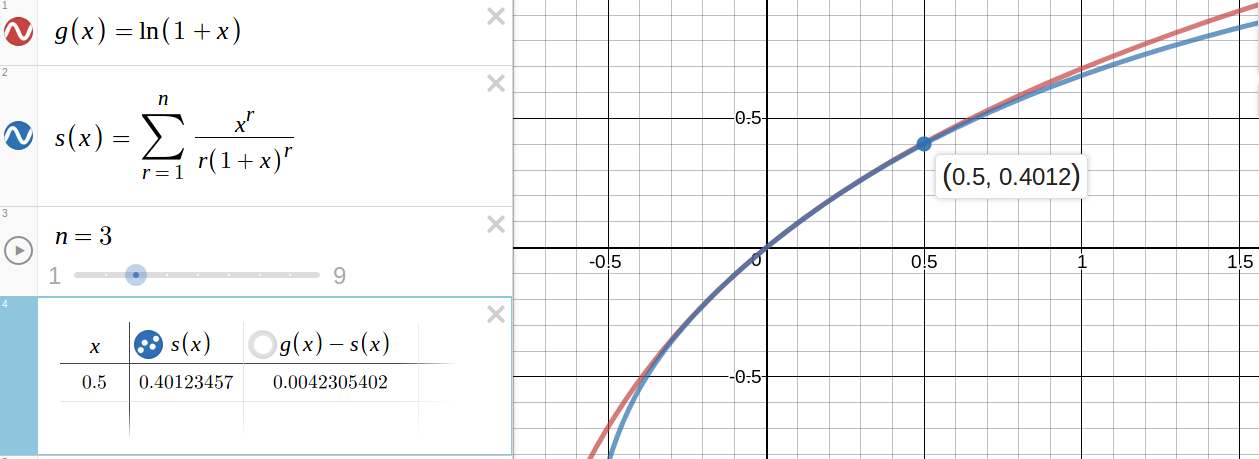
\includegraphics[width=12cm, height=4.7cm]{Selection_009.png}
\end{variableblock}

\end{frame}


\begin{frame}{Trigonometric functions ...}
\small
By considering $g(x) = \sin x$ the series expressions for the all trigonometric functions can be derived.

\begin{variableblock}{}{bg=green!10,fg=black}{}
\centering
\begin{tabular}{c c}

$\displaystyle{ \sin x = \frac{l_1}{\sqrt{l_1^2+(1-l_2)^2}}}$ & $\displaystyle{\cos x = \frac{1-l_2}{\sqrt{l_1^2+(1-l_2)^2}},} $\\

\\

$\displaystyle{\tan x =\frac{l_1}{1-l_2}}$ &
 $\displaystyle{\cot x = \frac{1-l_2}{l_1}, }$ \\ 
 
\\

$\displaystyle{ \sec x = \frac{\sqrt{l_1^2+(1-l_2)^2}}{1-l_2}}$ & $\displaystyle{ \csc x = \frac{\sqrt{l_1^2+(1-l_2)^2}}{l_1}}$.\\ 
\end{tabular}

\end{variableblock}
.\\

where $\displaystyle{ l_1=\sum_{r=0}^{\infty} \left( \dfrac{x^{4r+1}}{(4r+1)!} - \dfrac{x^{4r+3}}{(4r+3)!} \right)}$ and $\displaystyle{ l_2=\sum_{r=0}^{\infty} \left( \dfrac{x^{4r+2}}{(4r+2)!} - \dfrac{x^{4r+4}}{(4r+4)!} \right)}$.

\end{frame}

\begin{frame}{... Trigonometric functions ...}
\small
\begin{block}{}
Graphically, the convergence of $\displaystyle{\tan x =\frac{l_1}{1-l_2}}$ is as shown.
\end{block}

\begin{variableblock}{}{bg=blue!50,fg=black}{}
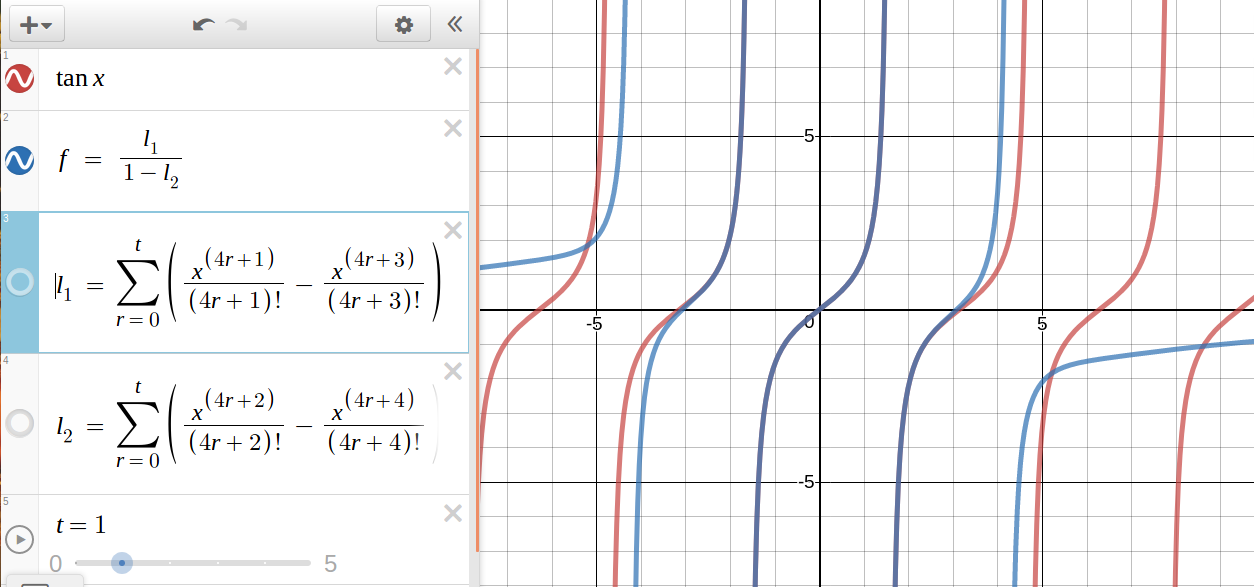
\includegraphics[width=12cm, height=5.5cm]{Selection_010.png}
\end{variableblock}
\end{frame}

\begin{frame}{... Trigonometric functions}
\small
\begin{block}{}
Similarly, the convergence of $\displaystyle{ \sin x = \frac{l_1}{\sqrt{l_1^2+(1-l_2)^2}}}$ is as shown.
\end{block}

\begin{variableblock}{}{bg=blue!50,fg=black}{}
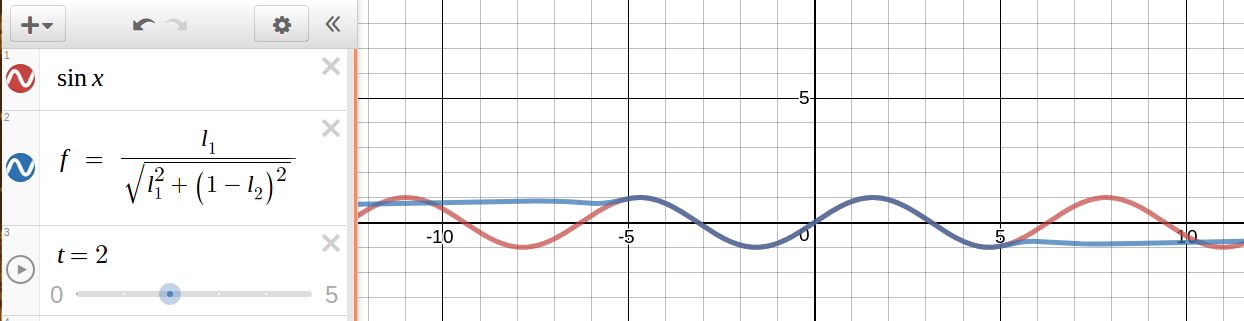
\includegraphics[width=12cm, height=4.5cm]{Selection_011.png}
\end{variableblock}
\end{frame}


\begin{frame}{}
    \begin{variableblock}{}{bg=green!50,fg=black}{}
    \begin{center}
    ~\\
        \huge{\textbf{ Result} }\\
    ~\\
    \end{center}
    \end{variableblock}

\end{frame}

\begin{frame}{$\pi$ ...}
\small

\begin{block}{}
The constant $\displaystyle{\pi}$ can be derived using an expression \eqref{TC1} by taking $g(x)=\tan ^{-1}x $ and $a=1$,
$$\tan ^{-1}x = \tan ^{-1}1 + \sum_{r=1}^{\infty} (-1)^{r-1} \frac{(x-1)^r}{r!} \left(  \frac{d^{r}}{dx^{r}} \tan ^{-1}x \right).$$
\end{block}

because $R_{n+1}(x) \rightarrow 0$ as $n \rightarrow \infty$.
The expansion of $\tan ^{-1}x $ is given by
\begin{eqnarray*}
\tan ^{-1} x = \sum_{k=0}^{\infty} (-1)^{k} \frac{x^{2k+1}}{2k+1},~~~~~~~ \textrm{where} ~~ |x|\leq 1
\end{eqnarray*}
and $\tan ^{-1}1 = \frac{\pi}{4}$. So,
$$\frac{\pi}{4} = \tan ^{-1}x - \sum_{r=1}^{\infty} \left[ (-1)^{r-1} \frac{(x-1)^r}{r!} \left( \frac{d^r}{dx^r} \sum_{k=0}^{\infty} (-1)^{k} \frac{x^{2k+1}}{2k+1} \right) \right].$$
\end{frame}

\begin{frame}{... $\pi$ ...}
\small
Now, the $r^{th}$ derivative of $\tan ^{-1} x$ is
\begin{eqnarray*}
\frac{d^{r}}{dx^{r}} \left( \sum_{k=0}^{\infty} (-1)^{k} \cdot \frac{x^{2k+1}}{2k+1} \right) = \sum_{k=\ceil{\frac{r-1}{2}}}^{\infty} \left[ \left\{ \prod_{p=1}^{r} ((2k+1)-(p-1)) \right\}  \right.\\
\cdot \left. \frac{(-1)^k \cdot x^{(2k+1)-r}}{2k+1} \right].
\end{eqnarray*}
So, the value of $\pi$ can be written as

\begin{variableblock}{}{bg=red!10,fg=black}{}
\begin{eqnarray*}
\pi = 4 \left[ \tan ^{-1} x + \sum_{r=1}^{\infty} \left[ (-1)^r \frac{(x-1)^r}{r!} \left[ \sum_{k=\ceil{\frac{r-1}{2}}}^{\infty} \left( \frac{(-1)^k}{2k+1} \cdot x^{(2k+1)-r} \cdot \right. \right. \right. \right. \\
\left. \left. \left. \left.  \left\{ \prod_{p=1}^{r} ((2k+1)-(p-1)) \right\} \right) \right] \right] \right]
\end{eqnarray*}
\end{variableblock}

for all $0<x<1$.
\end{frame}

\begin{frame}{... $\pi$}
\begin{block}{}
In the graph the value of $f$ converges to value of $\pi$ for $x \in (0,1).$ \\
\end{block}

\begin{variableblock}{}{bg=blue!50,fg=black}{}
\begin{center}
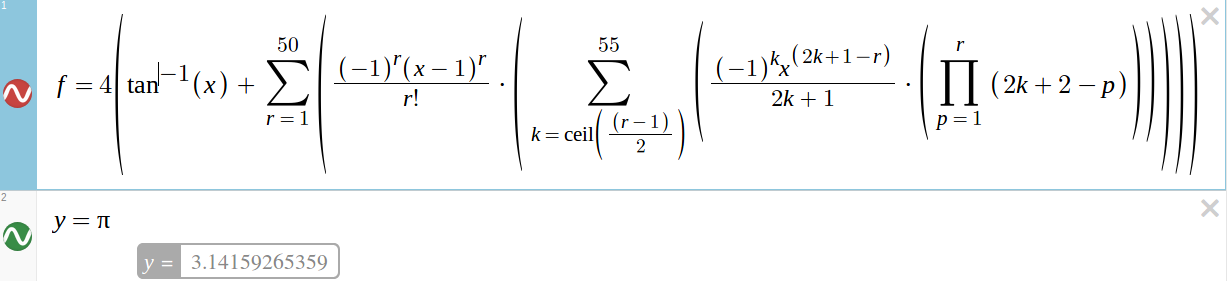
\includegraphics[width=12cm, height=2.3cm]{pie_formula.png}\\
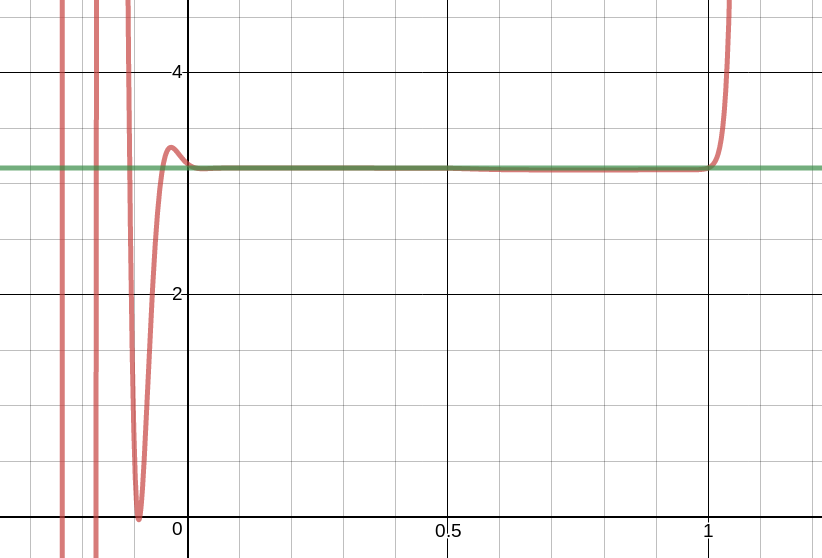
\includegraphics[width=12cm, height=3.8cm]{pie_graph.png}
\end{center}

\end{variableblock}

\end{frame}

% Placing a * after \section means it will not show in the
% outline or table of contents.
%\section*{Summary}

%\begin{frame}{Summary}
%  \begin{itemize}
%  \item
%    The \alert{first main message} of your talk in one or two lines.
  %\item
 %  \item
%    Perhaps a \alert{third message}, but not more than that.
 % \end{itemize}
  
 %  \item
  %   \begin{itemize}
%    \item
    %  Something you haven't solved.
   % \item
   %   Something else you haven't solved.
  %  \end{itemize}
 % \end{itemize}
%\end{frame}



% All of the following is optional and typically not needed. 
%\appendix
%\section<presentation>*{\appendixname}
%\subsection<presentation>*{For Further Reading}

\begin{frame}{References}%[allowframebreaks]


\begin{thebibliography}{1}
\bibitem{A}  A First Course in Mathematical Analysis by D Somasundaram and B Choudhary.
\bibitem{B} Graphs and error analysis are done using \url{www.desmos.com}
\bibitem{C} Introduction to numerical analysis by S.A. Mollah.
\bibitem{D} \url{https://en.wikipedia.org/wiki/Leibniz\_integral\_rule}
\bibitem{E} Numerical integration are done using inbuilt python command ``trapz". \url{https://docs.scipy.org/doc/numpy-1.13.0/reference/generated/numpy.trapz.html}

\end{thebibliography}
\vfill\eject


%  \frametitle<presentation>{For Further Reading}
    
%  \begin{thebibliography}{10}
    
%  \beamertemplatebookbibitems
  % Start with overview books.

%  \bibitem{Author1990}
%    A.~Author.
%    \newblock {\em Handbook of Everything}.
%    \newblock Some Press, 1990.
 
    
%  \beamertemplatearticlebibitems
  % Followed by interesting articles. Keep the list short. 

%  \bibitem{Someone2000}
%    S.~Someone.
%    \newblock On this and that.
%%    \newblock {\em Journal of This and That}, 2(1):50--100,
%    2000.
%  \end{thebibliography}
\end{frame}

\begin{frame}{}
\huge
    \begin{variableblock}{}{bg=green!50,fg=black}{}
    \begin{center}
    \color{orange}
        ~\\
        \textbf{\textit{ THANK YOU }}\\
        ~\\
        \dSmiley \dSmiley \dSmiley\\
        ~\\
    \end{center}
    \end{variableblock}
    
\end{frame}

\end{document}


